\section{Лекция 1: Разреженные матрицы}

\subsection{Форматы разреженных матриц}

Важно то, что их дофига. И разные хороши для разных задач.

Рассмотрм матрицу 

$$
M=
\begin{pmatrix}
1 & 0 & 0 & 0 & 3 & 0 & 9 & 0 \\
0 & 0 & 2 & 0 & 0 & -1 & 0 & 0 \\
0 & 0 & 0 & 7 & 0 & 0 & 0 & 0 \\
0 & 6 & 0 & 0 & 0 & 0 & 0 & 5 \\
0 & 3 & 4 & 0 & 0 & 0 & 0 & 0 \\
0 & 0 & 0 & 0 & 2 & 0 & 8 & 0 \\
0 & 0 & -3 & 0 & 0 & 0 & 0 & -7 \\
0 & 0 & 0 & 0 & -4 & 0 & 0 & 0 
\end{pmatrix}.
$$
В ней всего 15 ненулевыз элементов (NNZ(M) = 15).
Попробуем представить её в разных форматах.

\textbf{Покоординатный (COO).} Часто он же \textit{triple store}. Просто коллекция троек вида \textit(строка, столбец, значение) только для ненулевых элементов.
\begin{align*}
M_{\textit{COO}} = [&(0,0,1);(0,4,3);(0,6,9);(1,2,2);(1,5,-1);(2,3,7);(3,1,6);(3,7,5);(4,1,3);\\
           &(4,2,4);(5,4,2);(5,6,8); (6,2,-3);(2,7,-7);(7,4,-4) ]
\end{align*}

Потратили $3*NNZ(M)$ памяти.

Формат простой. Можно предварительно сортировать по столбцам или строкам. Достаточно просто удалять и добавлять элементы. Не самый оптимальный по доступу и по дополнительной памяти.

\textbf{Compressed row storage (CRS).} Заведём 3 массива: \textit{val} для хранения значений, \textit{col\_id} для хранения номера столбца, \textit{row\_ptr} для указателя на начало строки в \textit{col\_id}.

\begin{center}
$$
M_{\textit{CRS}} = (\textit{val},\textit{col\_id},\textit{row\_ptr} )
$$
\begin{tabular}{|c||c|c|c|c|c|c|c|c|c|c|c|c|c|c|c|}
\hline
val     & 1 & 3 & 9 & 2 & -1 & 7 & 6 & 5 & 3 & 4 & 2 & 8 & -3 & -7 & -4\\
col\_id & 0 & 4 & 6 & 2 & 5  & 3 & 1 & 7 & 1 & 2 & 4 & 6 & 2  & 7  & 4\\
\hline
\end{tabular}

\begin{tabular}{|c||c|c|c|c|c|c|c|c|}
\hline
row\_ptr & 0 & 3 & 5 & 6 & 8  & 10 & 12 & 14 \\
\hline
\end{tabular}
\end{center}

Потратили $2*NNZ(M) + n$ памяти. Сложнее построить, сложно удалять и добавлять. Достаточно просто последовательно обходить, лучше по памяти и по обращению к элементу. Наиболее часто встречается в современных библиотеках.

\textbf{Compressed column storage (CCS)} и \textbf{compressed dioganal storage (CDS).} Вариации на тему CRS. Второй --- для диоганальных матриц.

\textbf{Блочный CRS (CCS, CDS).} Когда мы знаем, что матрица имеет блочную структуру, а каждый блок --- разреженная матрица. Пример --- результат тензорного произведения.

\textbf{Quad-tree.}

Предположим, что $n=2^k$. Если это не так, то выравниваем нулями. После этого строим рекурсивно дерево: дели матрицу на 4 блока, корень --- это текущая матрица, листья --- 4 полученных блока. Если в блоке все элементы нули, то сразу рисуем лист типа \textit{(этот блок --- ноль)}, иначе продолжаем разбиение. И так до тех пор пока не получатся блоки из одного элемента.


$$
M=
\left[
\begin{array}{cccc|cccc}
1 & 0 & 0 & 0 & 3 & 0 & 9 & 0 \\
0 & 0 & 2 & 0 & 0 & -1 & 0 & 0 \\
0 & 0 & 0 & 7 & 0 & 0 & 0 & 0 \\
0 & 6 & 0 & 0 & 0 & 0 & 0 & 5 \\
\hline
0 & 3 & 4 & 0 & 0 & 0 & 0 & 0 \\
0 & 0 & 0 & 0 & 2 & 0 & 8 & 0 \\
0 & 0 & -3 & 0 & 0 & 0 & 0 & -7 \\
0 & 0 & 0 & 0 & -4 & 0 & 0 & 0 
\end{array}
\right]
$$

$$
M_{(0,0)}=
\left[
\begin{array}{cc|cc}
1 & 0 & 0 & 0 \\
0 & 0 & 2 & 0 \\
\hline
0 & 0 & 0 & 7 \\
0 & 6 & 0 & 0 \\
\end{array}
\right],
M_{(0,1)}=
\left[
\begin{array}{cc|cc}
3 & 0 & 9 & 0 \\
0 & -1 & 0 & 0 \\
\hline
0 & 0 & 0 & 0 \\
0 & 0 & 0 & 5 \\ 
\end{array}
\right]
$$

$$
M_{(1,0)}=
\left[
\begin{array}{cc|cc}
0 & 3 & 4  & 0 \\
0 & 0 & 0  & 0 \\
\hline
0 & 0 & -3 & 0 \\
0 & 0 & 0  & 0  
\end{array}
\right],
M_{(1,1)}=
\left[
\begin{array}{cc|cc}
 0  & 0 & 0 & 0 \\
 2  & 0 & 8 & 0 \\
 \hline
 0  & 0 & 0 & -7 \\
 -4 & 0 & 0 & 0 
\end{array}
\right]
$$

$$
M_{(0,0)(0,0)}=
\left[
\begin{array}{c|c}
1 & 0 \\
\hline
0 & 0 
\end{array}
\right],
M_{(0,0)(0,1)}=
\left[
\begin{array}{c|c}
0 & 0 \\
\hline
2 & 0 
\end{array}
\right],
M_{(0,0)(1,0)}=
\left[
\begin{array}{c|c}
0 & 0 \\
\hline
0 & 6 
\end{array}
\right],
M_{(0,0)(1,1)}=
\left[
\begin{array}{c|c}
0 & 7 \\
\hline
0 & 0 
\end{array}
\right]
$$

$$
M_{(0,1)(0,0)}=
\left[
\begin{array}{c|c}
3 & 0  \\
\hline
0 & -1 \\
\end{array}
\right],
M_{(0,1)(0,1)}=
\left[
\begin{array}{c|c}
9 & 0 \\
\hline
0 & 0 \\
\end{array}
\right],
M_{(0,1)(1,1)}=
\left[
\begin{array}{c|c}
0 & 0 \\
\hline
0 & 5 \\ 
\end{array}
\right]
$$

$$
M_{(1,0)(0,0)}=
\left[
\begin{array}{c|c}
0 & 3 \\
\hline
0 & 0 
\end{array}
\right],
M_{(1,0)(0,1)}=
\left[
\begin{array}{c|c}
4  & 0 \\
\hline
0  & 0 
\end{array}
\right],
M_{(1,0)(1,1)}=
\left[
\begin{array}{c|c}
 -3 & 0 \\
 \hline
 0  & 0  
\end{array}
\right]
$$

$$
M_{(1,1)(0,0)}=
\left[
\begin{array}{c|c}
 0  & 0 \\
 \hline
 2  & 0 
\end{array}
\right],
M_{(1,1)(0,1)}=
\left[
\begin{array}{c|c}
0 & 0 \\
\hline
8 & 0 
\end{array}
\right],
M_{(1,1)(1,0)}=
\left[
\begin{array}{c|c}
 0  & 0\\
 \hline
 -4 & 0
\end{array}
\right],
M_{(1,1)(1,1)}=
\left[
\begin{array}{c|c}
 0  & -7 \\
 \hline
 0 & 0 
\end{array}
\right]
$$

\resizebox{.99\textwidth}{!}{
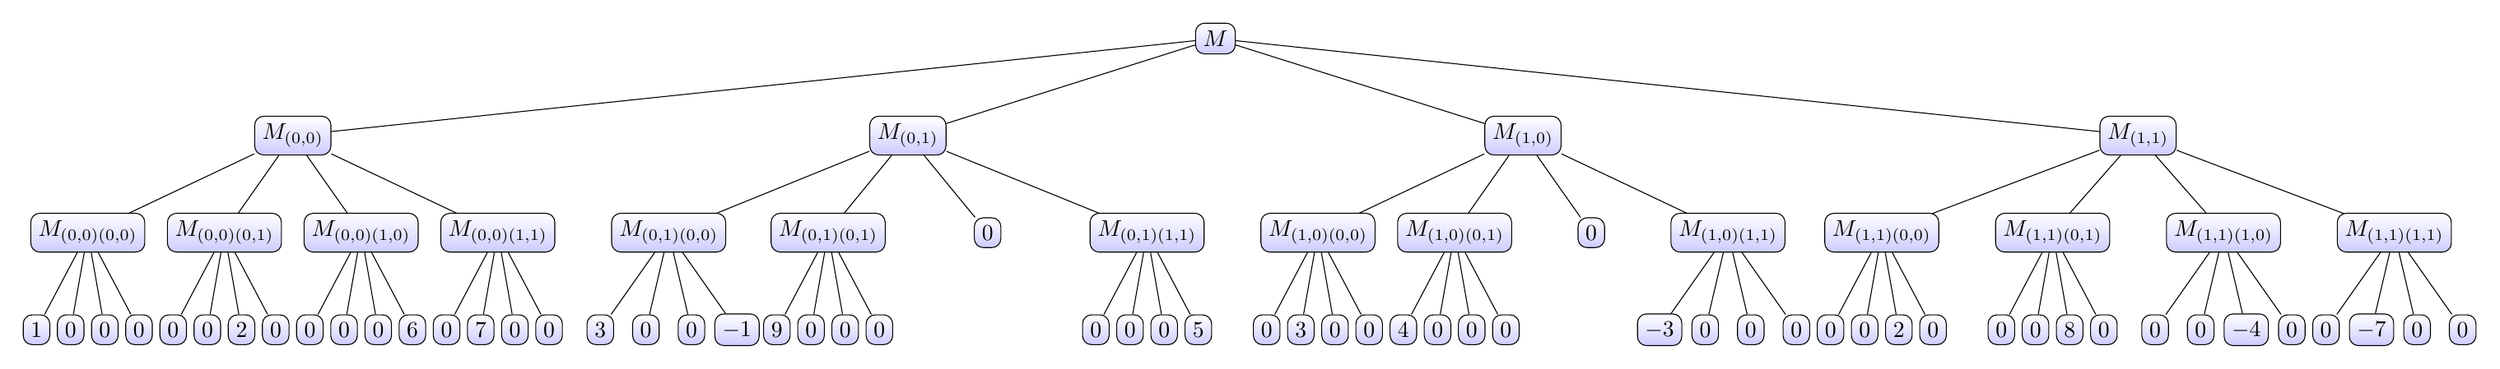
\begin{tikzpicture}[sibling distance=27em,
  every node/.style = {shape=rectangle, rounded corners,
    draw, align=center,
    top color=white, bottom color=blue!20}]]
  \node {$M$}
    child {[sibling distance=6em] 
        node {$M_{(0,0)}$} 
        child { [sibling distance=1.5em] 
            node {$M_{(0,0)(0,0)}$} 
            child {node {$1$}}
            child {node {$0$}}
            child {node {$0$}}
            child {node {$0$}} }
        child { [sibling distance=1.5em]
            node {$M_{(0,0)(0,1)}$} 
            child {node {$0$}}
            child {node {$0$}}
            child {node {$2$}}
            child {node {$0$}} }
        child { [sibling distance=1.5em]
            node {$M_{(0,0)(1,0)}$}
            child {node {$0$}}
            child {node {$0$}}
            child {node {$0$}}
            child {node {$6$}} }
        child { [sibling distance=1.5em]
            node {$M_{(0,0)(1,1)}$}
            child {node {$0$}}
            child {node {$7$}}
            child {node {$0$}}
            child {node {$0$}} } }
    child { [sibling distance=7em] 
        node {$M_{(0,1)}$}
        child { [sibling distance=2em] 
            node {$M_{(0,1)(0,0)}$}
            child {node {$3$}}
            child {node {$0$}}
            child {node {$0$}}
            child {node {$-1$}} }
        child { [sibling distance=1.5em] 
            node {$M_{(0,1)(0,1)}$}
            child {node {$9$}}
            child {node {$0$}}
            child {node {$0$}}
            child {node {$0$}} }
        child { node {$0$} }
        child { [sibling distance=1.5em] 
            node {$M_{(0,1)(1,1)}$}
            child {node {$0$}}
            child {node {$0$}}
            child {node {$0$}}
            child {node {$5$}} } }
    child { [sibling distance=6em]
        node {$M_{(1,0)}$} 
        child { [sibling distance=1.5em] 
            node {$M_{(1,0)(0,0)}$}
            child {node {$0$}}
            child {node {$3$}}
            child {node {$0$}}
            child {node {$0$}} }
        child { [sibling distance=1.5em] 
            node {$M_{(1,0)(0,1)}$}
            child {node {$4$}}
            child {node {$0$}}
            child {node {$0$}}
            child {node {$0$}} }
        child { node {$0$} }
        child { [sibling distance=2em] 
            node {$M_{(1,0)(1,1)}$} 
            child {node {$-3$}}
            child {node {$0$}}
            child {node {$0$}}
            child {node {$0$}} } }
    child { [sibling distance=7.5em]
        node {$M_{(1,1)}$} 
        child { [sibling distance=1.5em] 
            node {$M_{(1,1)(0,0)}$}
            child {node {$0$}}
            child {node {$0$}}
            child {node {$2$}}
            child {node {$0$}} }
        child { [sibling distance=1.5em] 
            node {$M_{(1,1)(0,1)}$}
            child {node {$0$}}
            child {node {$0$}}
            child {node {$8$}}
            child {node {$0$}} }
        child { [sibling distance=2em] 
            node {$M_{(1,1)(1,0)}$}
            child {node {$0$}}
            child {node {$0$}}
            child {node {$-4$}}
            child {node {$0$}} }
        child { [sibling distance=2em] 
            node {$M_{(1,1)(1,1)}$}
            child {node {$0$}}
            child {node {$-7$}}
            child {node {$0$}}
            child {node {$0$}} } };
\end{tikzpicture}
}

Относительно сложно построить, легко разделить на части (хорошо для распределённых вычислений), достаточно быстрый доступ к элементу, простой рекурсивный алгоритм перемножения.

Часто используется в композиции с CRS или другими форматами: до какого-то момента строим дередо, а потом в листьях храним сравнительно большие подматрицы в CRS.

\subsection{Умножение разреженных матриц}

Временная сложность оценивается относительно количества ненулевых элементов (NNZ) либо во входных матрицах, либо в выходной матрице, либо и там и там.